\begin{figure}[h] 
\centering 
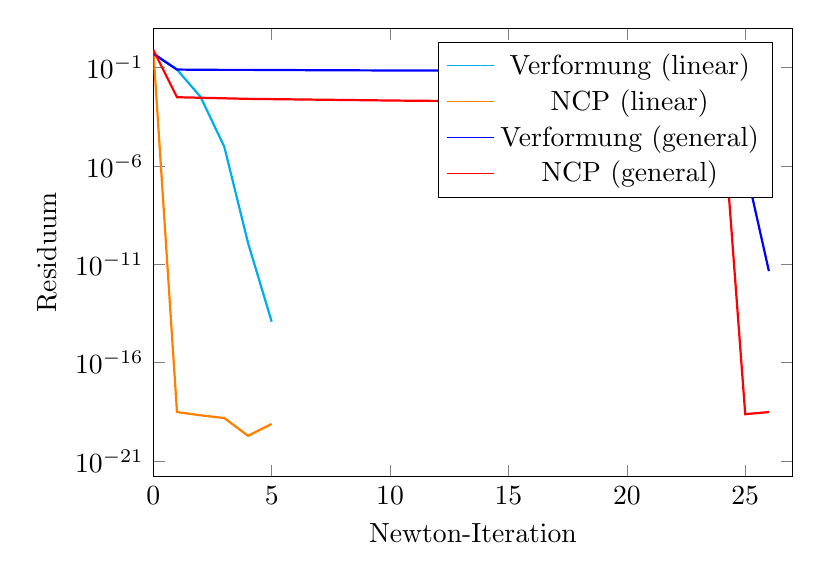
\begin{tikzpicture}[every plot/.append style={thick}] 
\begin{axis}[ 
label style={font=\normalsize}, 
xlabel={Newton-Iteration}, 
ylabel={Residuum}, 
xmin=0, xmax=27, 
ymode=log, 
ymin=0, ymax=10, 
width=0.8\textwidth, 
height=0.6\textwidth, 
legend pos=north east, 
legend style={cells={align=left}}, 
grid style=dashed, 
] 
\addplot[ 
color=cyan, 
] 
coordinates { 
(0, 5.09e-01)(1, 7.93e-02)(2, 3.17e-03)(3, 9.26e-06)(4, 1.23e-10)(5, 1.21e-14)}; 
\addlegendentry{Verformung (linear)} 
\addplot[ 
color=orange, 
] 
coordinates { 
(0, 7.92e-01)(1, 3.09e-19)(2, 2.11e-19)(3, 1.53e-19)(4, 1.92e-20)(5, 7.67e-20)}; 
\addlegendentry{NCP (linear)} 
\addplot[ 
color=blue, 
] 
coordinates { 
(0, 5.09e-01)(1, 7.93e-02)(2, 7.72e-02)(3, 7.63e-02)(4, 7.65e-02)(5, 7.54e-02)(6, 7.44e-02)(7, 7.35e-02)(8, 7.27e-02)(9, 7.20e-02)(10, 7.15e-02)(11, 7.13e-02)(12, 7.08e-02)(13, 7.04e-02)(14, 7.02e-02)(15, 9.07e-02)(16, 1.39e-01)(17, 1.36e-01)(18, 3.40e-02)(19, 2.98e-02)(20, 8.20e-03)(21, 3.22e-03)(22, 1.62e-03)(23, 9.55e-03)(24, 4.70e-04)(25, 1.05e-06)(26, 4.52e-12)}; 
\addlegendentry{Verformung (general)} 
\addplot[ 
color=red, 
] 
coordinates { 
(0, 7.92e-01)(1, 3.11e-03)(2, 2.92e-03)(3, 2.74e-03)(4, 2.57e-03)(5, 2.49e-03)(6, 2.41e-03)(7, 2.33e-03)(8, 2.26e-03)(9, 2.19e-03)(10, 2.12e-03)(11, 2.06e-03)(12, 2.02e-03)(13, 1.99e-03)(14, 1.96e-03)(15, 7.22e-03)(16, 7.11e-03)(17, 7.00e-03)(18, 6.88e-03)(19, 6.77e-03)(20, 6.84e-03)(21, 6.73e-03)(22, 6.83e-03)(23, 6.84e-03)(24, 3.04e-03)(25, 2.42e-19)(26, 3.07e-19)}; 
\addlegendentry{NCP (general)} 
\end{axis} 
\end{tikzpicture} 
\caption{Residuen des Stoffgesetzes 'St.Venant' mit Hinderniss 'Hut' und 2178 Freiheitsgraden für die Verschiebung.} 
\label{fiq:St.Venant_Hut_level4} 
\end{figure} 
